\section{Communication Protocols}
\label{sec:comm_prot}

This section provides a brief overview of the different communication protocols used in this work.

\subsection{UART}
\label{sec:comm_uart}

Universal Asynchronous Receiver-Transmitter (UART) is a serial, asynchronous communication protocol which uses two wires (a receiver (RX) and a transmitter (TX)) to transfer data between two devices \cite{uart}. UART does not require a shared clock signal as it is asynchronous, however the devices communicating have to use the rate of data transfer, called the baud rate, for communication to be possible. A UART frame consists of a starting bit, a number of data bits (usually 8), and a stop it, as shown in Figure \ref{fig:uart_frame}.

\begin{figure}[H]
    \centering
    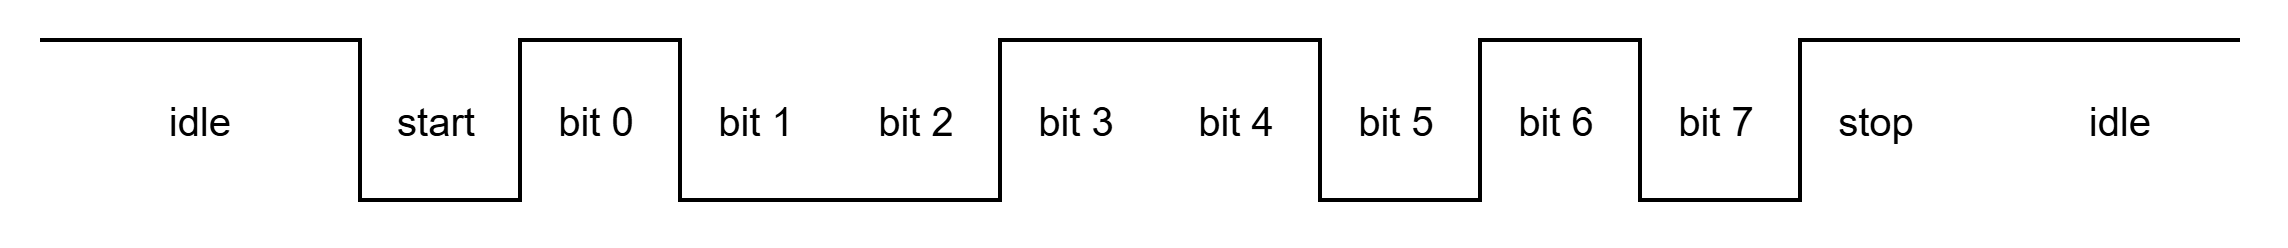
\includegraphics[width =1.0\textwidth]{Figures/uart_transmission.png}
    \caption{Example of UART fram, with starting bit, 8 data bits and stop bit.}
    \label{fig:uart_frame}
\end{figure}
\subsection{SPI}
\label{sec:comm_spi}

Serial Peripheral Interface (SPI) is a synchronous serial protocol which uses a master-slave architecture \cite{spi}. The master generates a common clock signal (SCLK), and selects which slave to communicate with through a chip select signal (CS). Data is exchanged in two directions at once using two data lines called MOSI (master out, slave in) and MISO (master in, slave out). A connection between a master device and a slave device is shown in Figure \ref{fig:spi_connection
}.


\begin{figure}[H]
\centering
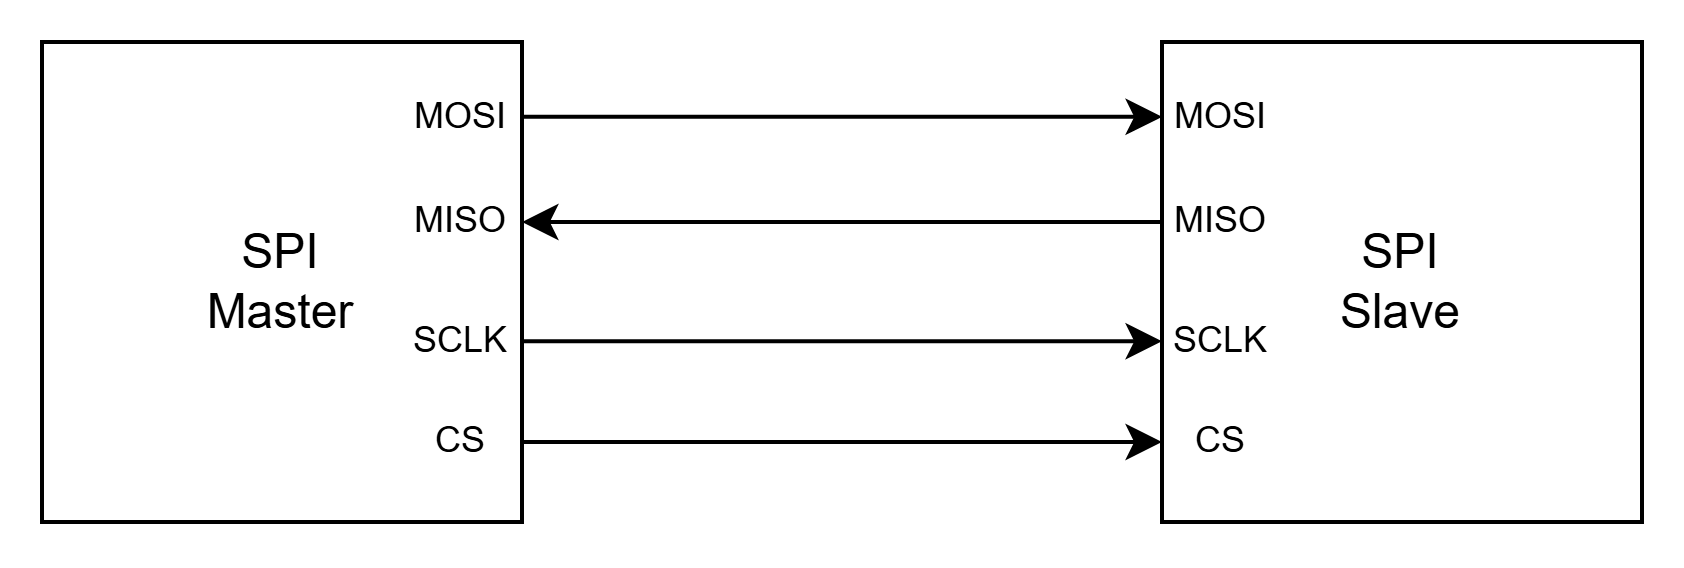
\includegraphics[width=1\textwidth]{Figures/spi_conn.png}
\caption{SPI connection between a master and a single slave.}
\label{fig:spi_connection}
\end{figure}

\subsection{Wishbone}
\label{sec:comm_wishbone}

Wishbone is an open source bus created to let different cores or IPs communicate inside of a chip, like on an FPGA or ASIC \cite{peterson_wishbone}. In short, it uses a master-slave architecture, and uses a handshake system where a master requests a slave to perform an action (read/write), and waits for the slave to communicate wether or not it ready to perform/has completed the action. It features various signals, like a cycle signal (CYC) letting device claim the Wishbone bus, however in depth understanding is not needed for this work. A more in depth explanation is given in \cite{peterson_wishbone}.


\subsection{AXI4}
\label{sec:comm_axi4}

The Advanced eXtensible Inferface (AXI) is an on-chip bus protocol similar to Wishbone, created by ARM \cite{wade2016axi}. While not open source, it is royalty-free and freely available. It has also been adopted by Xilinx as the main communication bus in their products \cite{amd_ar1053914}. It features a handshake system like in Wishbone, as well as the master-slave architecture. For communication it uses five channels, Read Address (AR), Read Data (R), Write Address (AW), Write Data (W), and Write Response (B). Each channel is independent of the others, which opens up the possibility for parallel read and write operations between devices. Examples of AXI read and AXI write operations are shown in Figure \ref{fig:axi_read} and \ref{fig:axi_write}.

\begin{figure}[H]
\centering
\begin{minipage}{.48\textwidth}
  \centering
  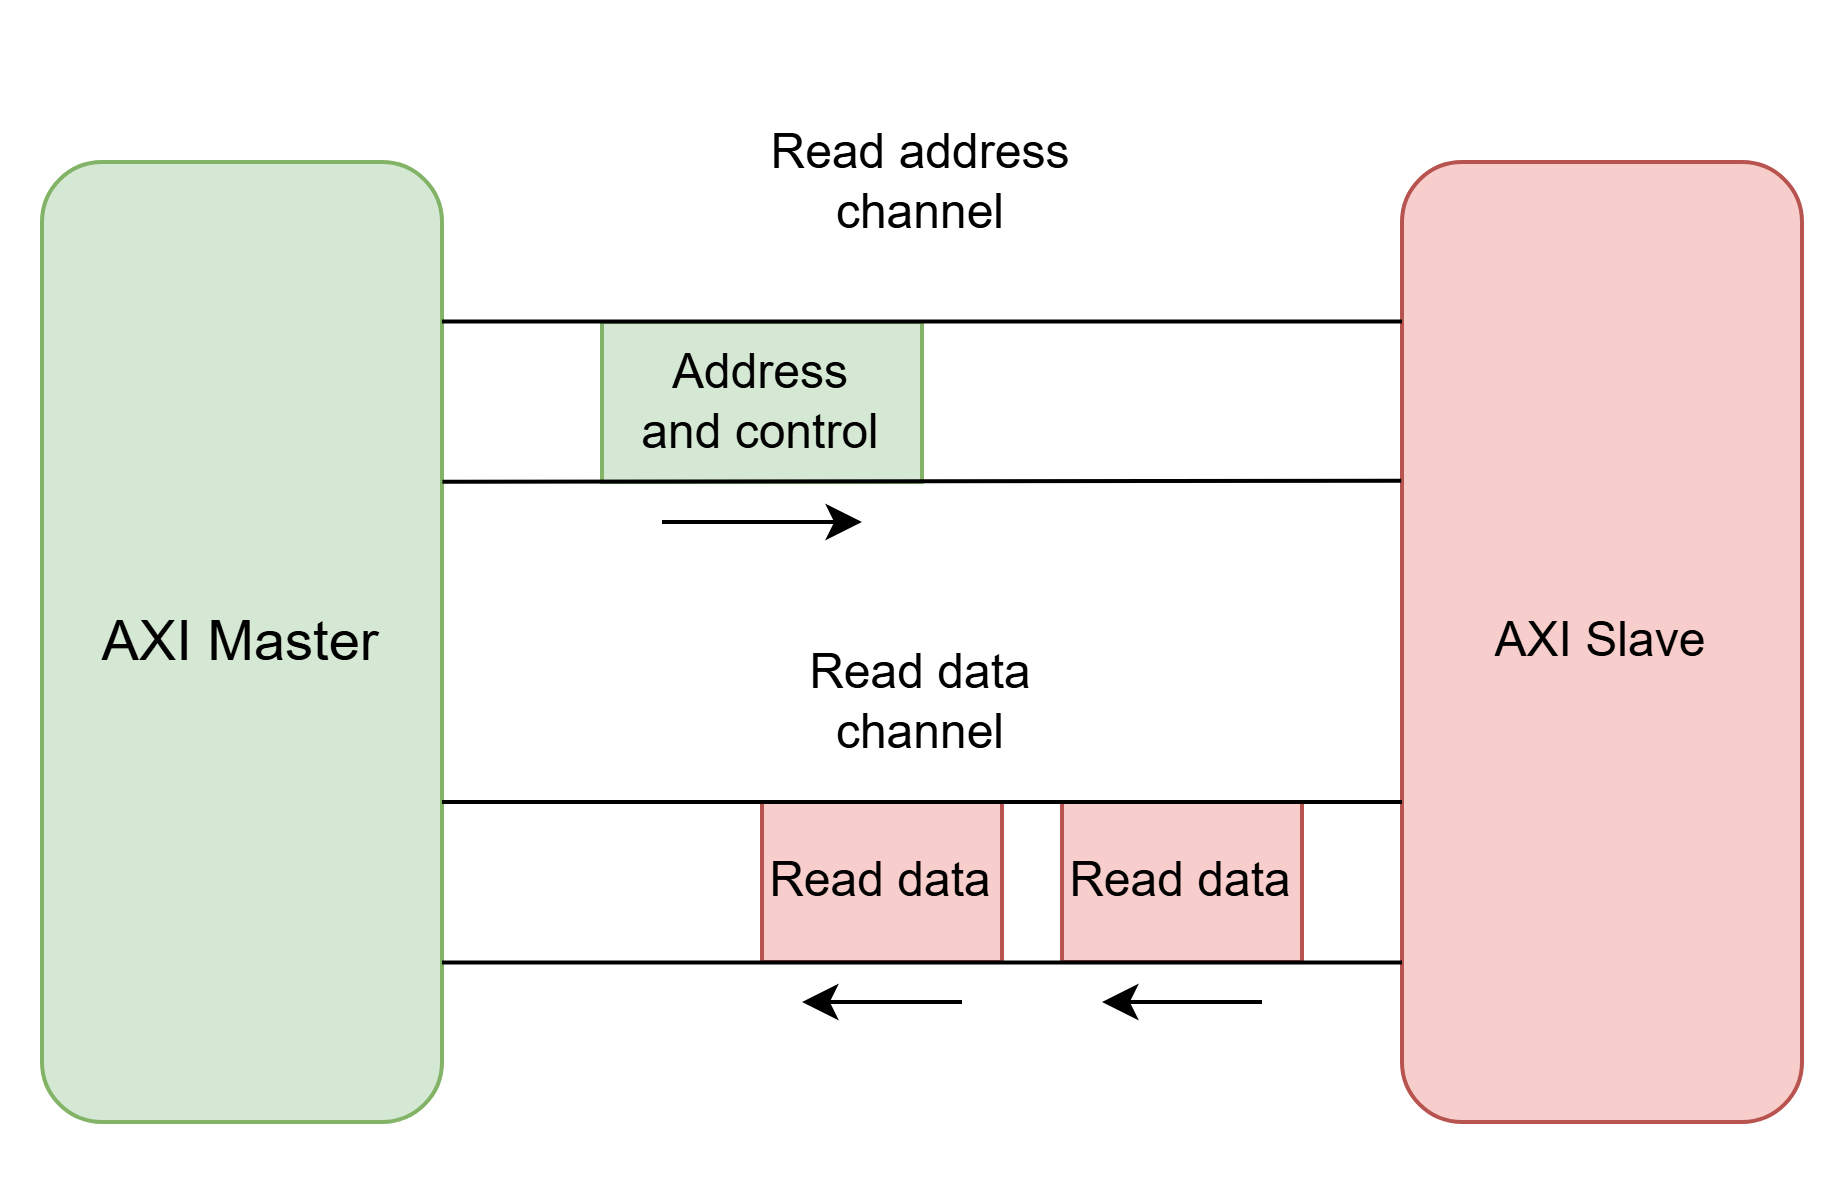
\includegraphics[width=1\textwidth]{Figures/axi_read.png}
  \caption{AXI read \cite{amd_ar1053914}.}
  \label{fig:axi_read}
\end{minipage}\hfill
\begin{minipage}{.48\textwidth}
    \centering
    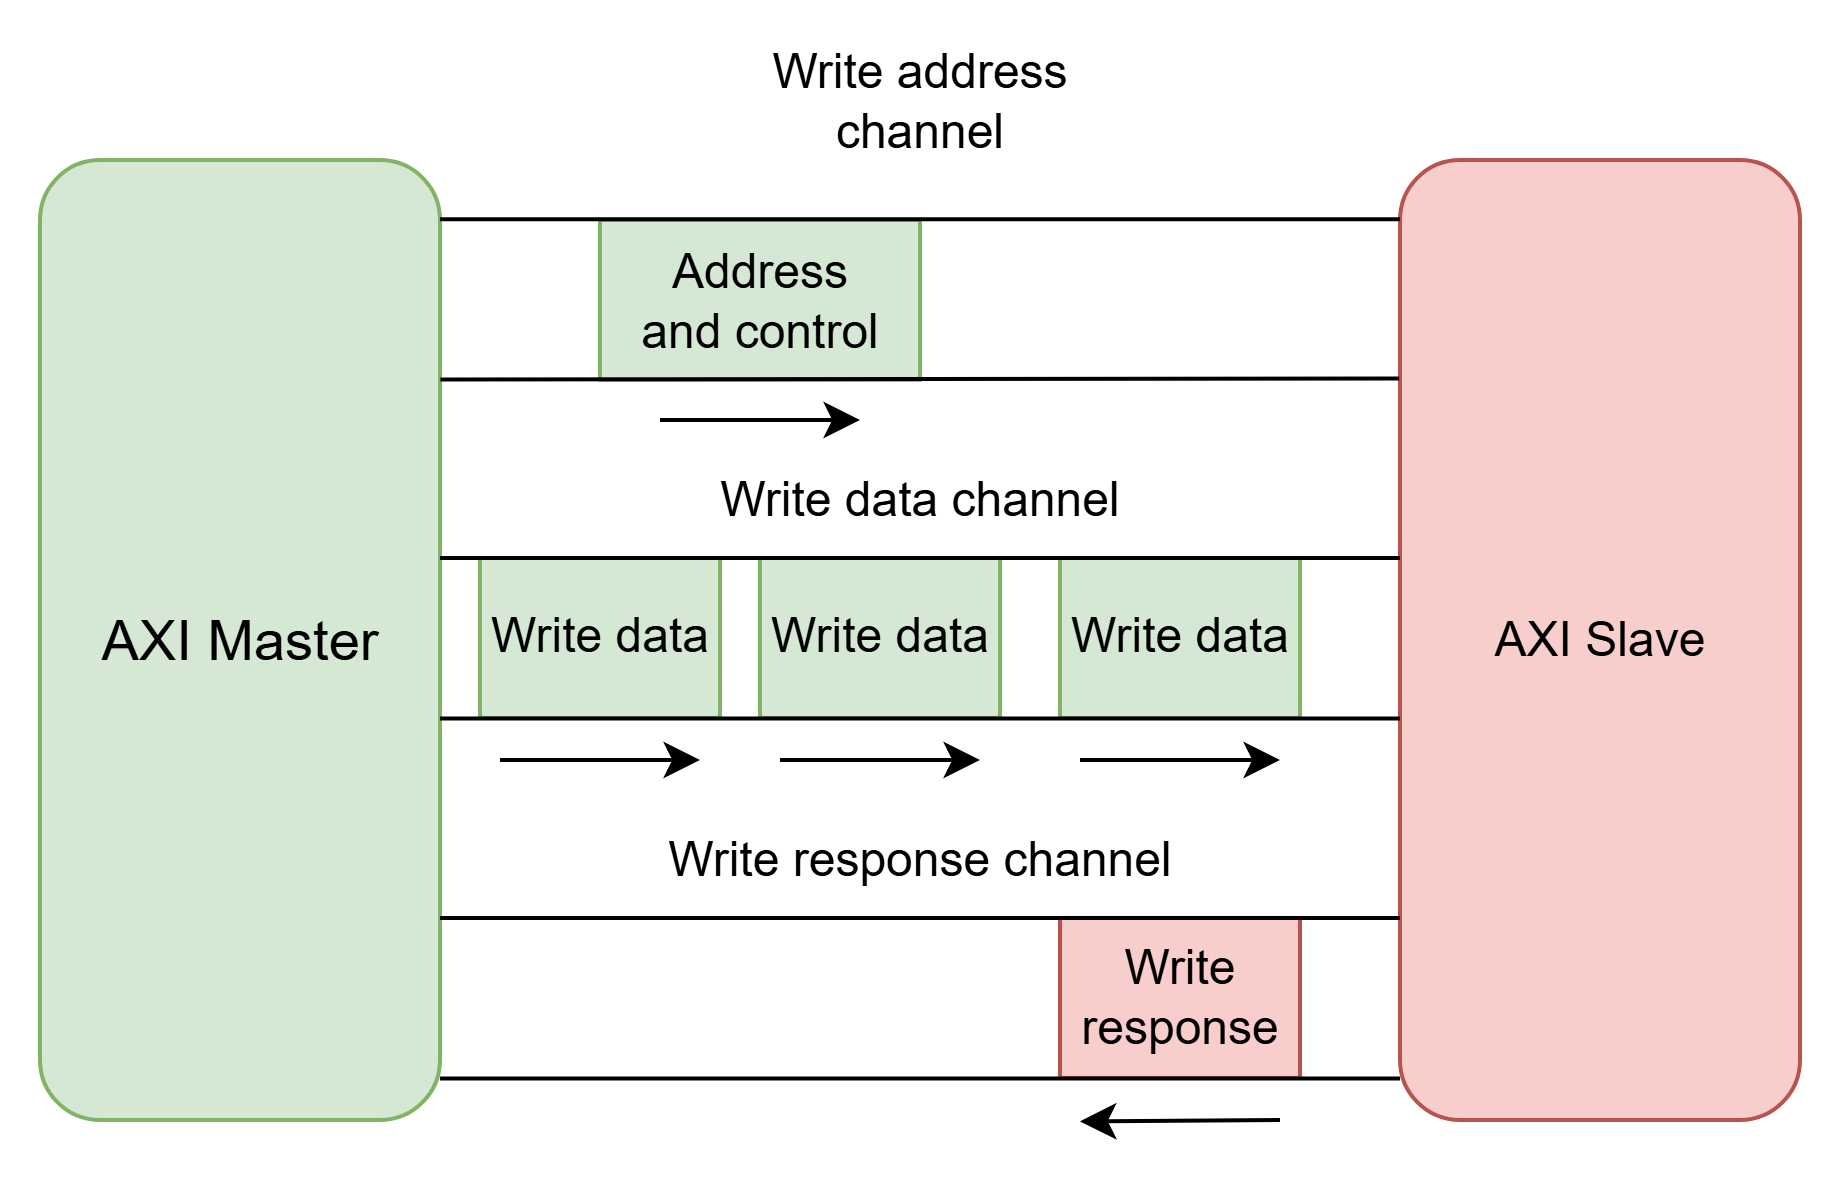
\includegraphics[width =1\textwidth]{Figures/axi_write.png}
    \caption{AXI write \cite{amd_ar1053914}.}
    \label{fig:axi_write}
\end{minipage}
\end{figure}


% \begin{figure}[H]
%     \centering
%     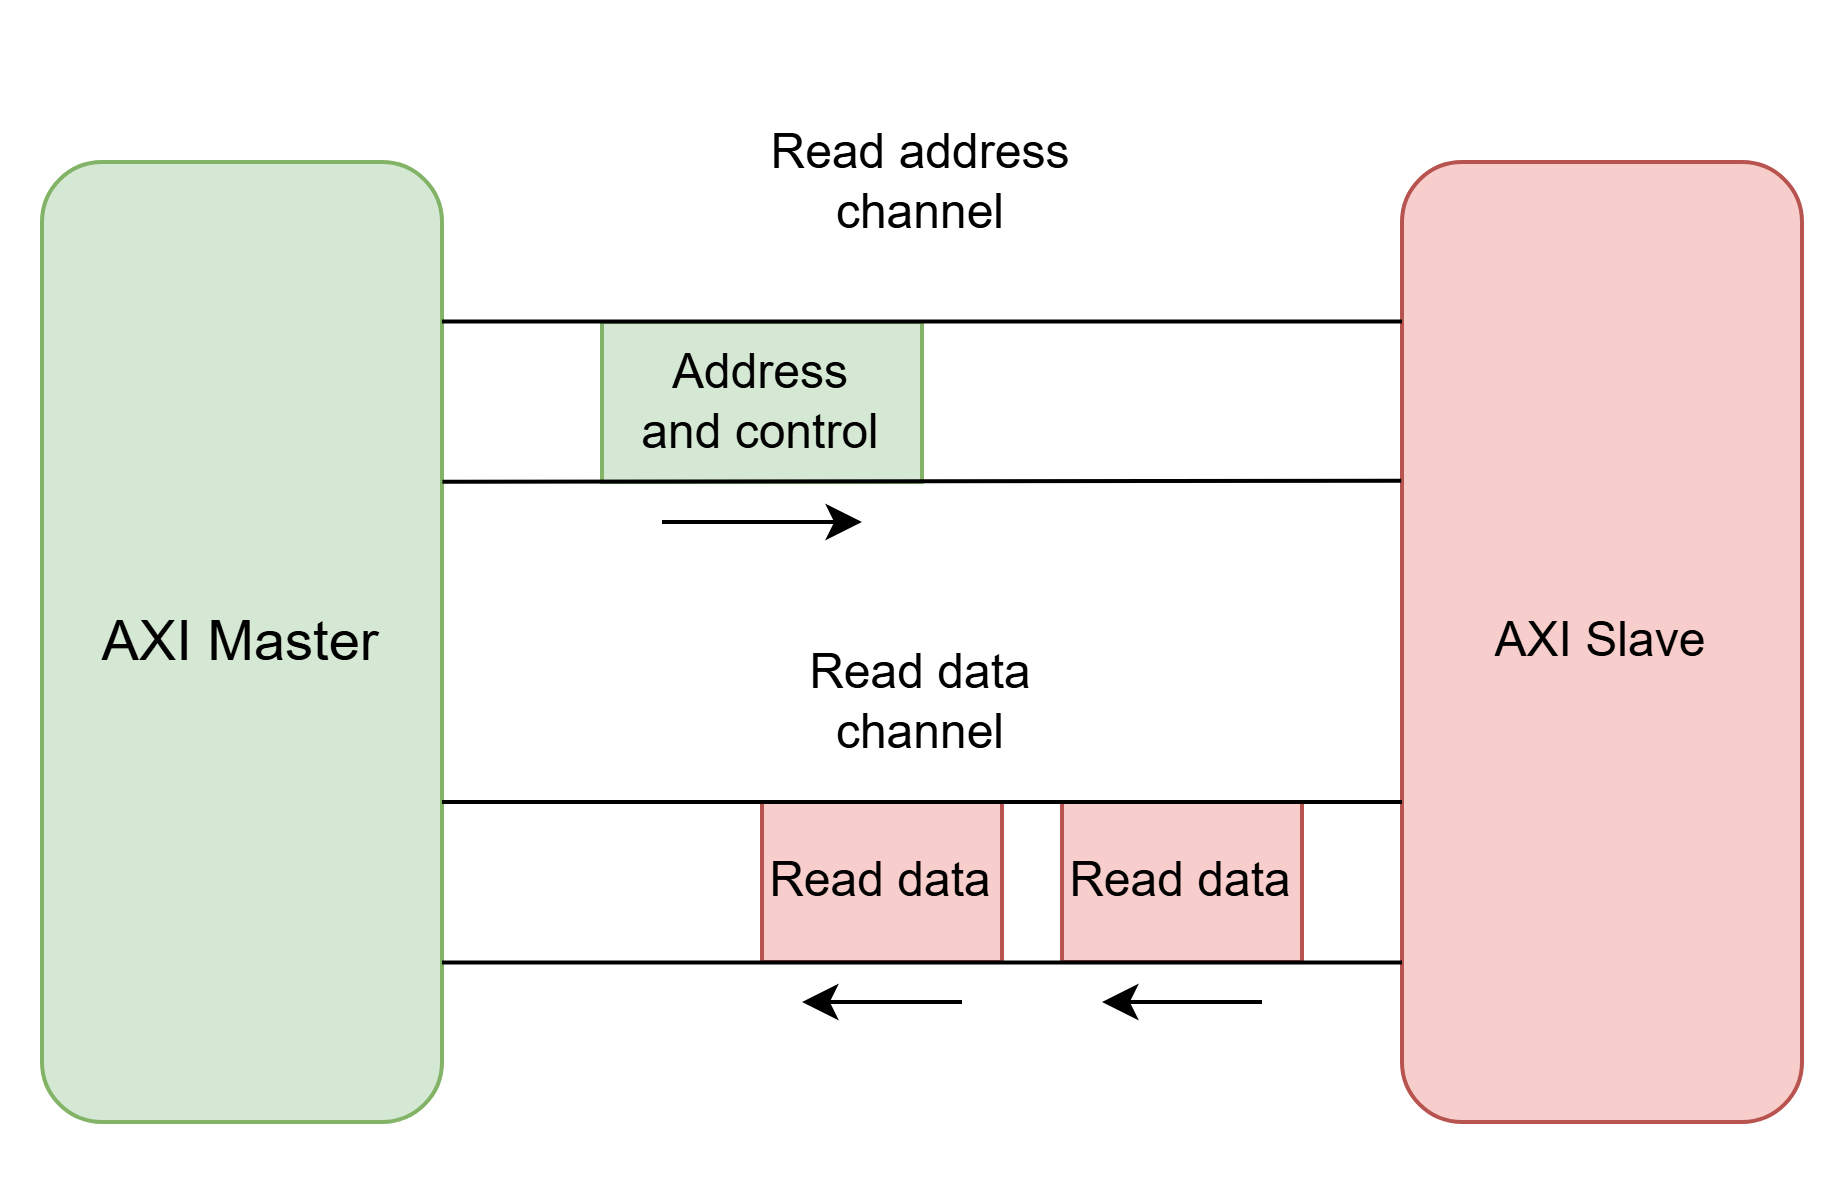
\includegraphics[width =0.7\textwidth]{Figures/axi_read.png}
%     \caption{AXI read operation \cite{amd_ar1053914}.}
%     \label{fig:axi_read}
% \end{figure}
% \begin{figure}[H]
%     \centering
%     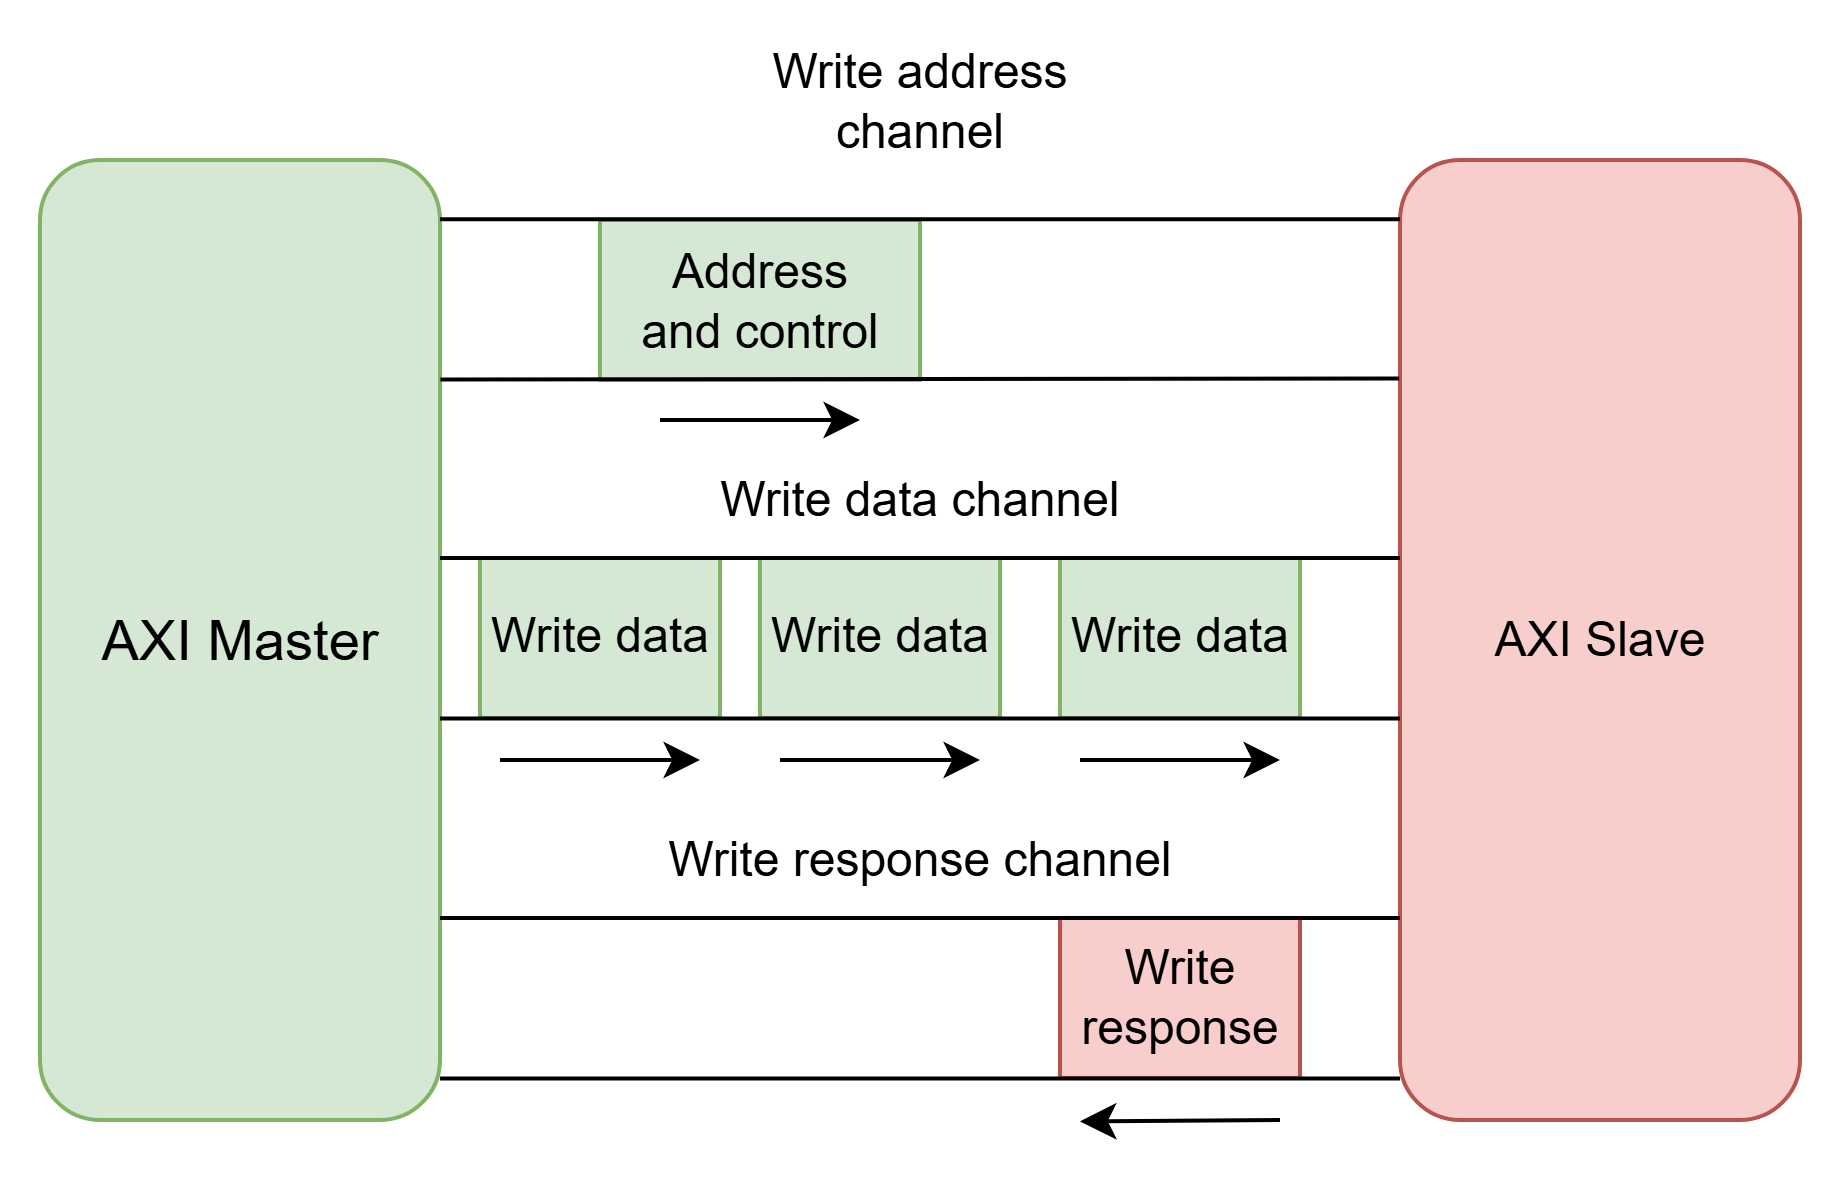
\includegraphics[width =0.7\textwidth]{Figures/axi_write.png}
%     \caption{AXI write operation \cite{amd_ar1053914}.}
%     \label{fig:axi_write}
% \end{figure}